\chapter{Теоретические результаты}
\label{chapter2}

В данной главе рассматривается теоритические аспекты разработки фремворка. Будет преведена общая схема фремворка, описаны основные модули. Также будет рассказано о ходе выполнения тестов и преведены примеры использования работы на примере jUnit тестов. 

\section{Общая схема работы} 

Общая схема работы фремворка показана на рисунке \ref{fig:allure}. Рассмотрим подробнее назначение отдельных частей.

\begin{figure}[htb]
\centering
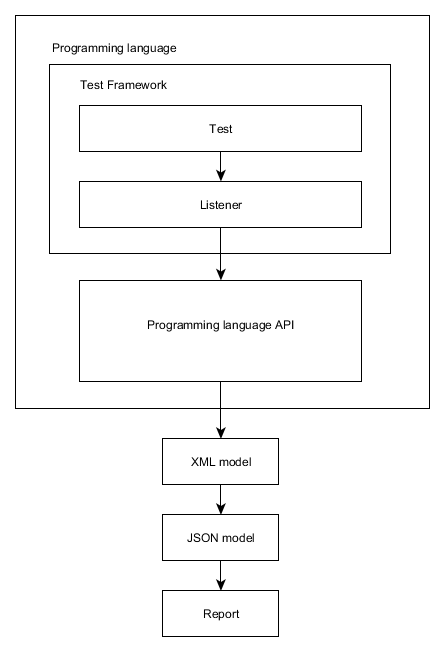
\includegraphics[height=160mm]{structure.png}
\caption{Общая схема фремворка Allure}
\label{fig:allure}
\end{figure}

\subsection{Listener}

Для большинства тестовых фремворков xUnit есть возможность подключить листенер для сбора информации о ходе тестов. Мало того, подключение листенера, как правило, вынесено на уровень конфигурации запуска, что полностью удавлетворяет требованиям работы. Для адаптации тестового фремворка достаточно реализовать тест листенер используя соответсвующее API языка программирования.

Однако стоит заметить, что не всю необходимую информацию о ходе теста можно собрать используя листенер, так как он оперирует терминологией xUnit. Сбор остальной информации о тестах, например информацию о пройденных шагах и сделанных аттачментах, будет реализован на уровне API языка программирования.

\subsection{Programming language API}

API для языка программирования представляет из себя набор обработчиков событий и сами события, используя которые можно полностью описать жизненный цикл теста. Программный инетрфейс содержит в себе следующие события:

\begin{itemize}
\item начало/конец тестового запуска;
\item начало/конец тест суита;
\item начало/конец тест кейса;
\item начало/конец шага;
\item сохранение аттачмента;
\item добавление параметров запуска/тест суита/тест кейса;
\item изменение статуса теста/шага;
\item добавление пометок к тесту.
\end{itemize}

С использованием API для языка программирования сильно упрощается написание и поддержка листнеров для тестовых фремворков. Вся собранная информация о ходе тестов сохраняется в XML модель. 

\subsection{XML model}

Собранная о тесте информация серелизуется в виде XML файлов. Для каждого теста создается свой файл. Сохраняются только те данные, которые нельзя синтезировать, что упрощает реализацию и поддержку интерфейса для языка программирования. Простейший пример сохранненной информации об одном тесте:

\begin{lstlisting}[style=XML]
<?xml version="1.0" encoding="UTF-8" standalone="yes"?>
<ns2:test-suite xmlns:ns2="urn:model.allure.qatools.yandex.ru" start="1400681607876" stop="1400681627123">
    <name>my.company.SampleTest</name>
    <test-cases>
        <test-case start="1400681608883" stop="1400681608891" status="passed">
            <name>test_pass</name>
        </test-case>
    </test-cases>
    <labels/>
</ns2:test-suite>
\end{lstlisting}

\subsection{JSON model}

На следующем этапе данные конвертируются 